
% ----------------------------------------------------------------------
%  Set the document class
% ----------------------------------------------------------------------
\documentclass[11pt,a4paper,twoside]{article}

% ----------------------------------------------------------------------
% Define external packages, language, margins, fonts and new commands
% ----------------------------------------------------------------------
%\input{preamble} 
\usepackage[utf8]{inputenc}   % <<<<< Linux
\usepackage[english]{babel} % <<<<< English
\usepackage{notoccite}
\usepackage[skip=0.5\baselineskip]{caption}
\hyphenation{GTKWave}
\usepackage{listings}
\usepackage[all]{nowidow}

%blind text
\usepackage{lipsum}

\usepackage{graphicx}
\graphicspath{{./}{../../figlib/}{../mat/}{../sim/}}
\def\FontLn{% 16 pt normal
  \usefont{T1}{phv}{m}{n}\fontsize{16pt}{16pt}\selectfont}
\def\FontLb{% 16 pt bold
  \usefont{T1}{phv}{b}{n}\fontsize{16pt}{16pt}\selectfont}
\def\FontMn{% 14 pt normal
  \usefont{T1}{phv}{m}{n}\fontsize{14pt}{14pt}\selectfont}
\def\FontMb{% 14 pt bold
  \usefont{T1}{phv}{b}{n}\fontsize{14pt}{14pt}\selectfont}
\def\FontSn{% 12 pt normal
  \usefont{T1}{phv}{m}{n}\fontsize{12pt}{12pt}\selectfont}

% Use Arial font as default
%
\renewcommand{\rmdefault}{phv}
\renewcommand{\sfdefault}{phv}
\usepackage{geometry}	
\geometry{verbose,tmargin=2.5cm,bmargin=2.5cm,lmargin=2.5cm,rmargin=2.5cm}

%\usepackage{setspace}
%\renewcommand{\baselinestretch}{1.5}

\usepackage[pdftex]{hyperref} % enhance documents that are to be
                              % output as HTML and PDF
\hypersetup{colorlinks,       % color text of links and anchors,
                              % eliminates borders around links
%            linkcolor=red,    % color for normal internal links
            linkcolor=black,  % color for normal internal links
            anchorcolor=black,% color for anchor text
%            citecolor=green,  % color for bibliographical citations
            citecolor=black,  % color for bibliographical citations
%            filecolor=magenta,% color for URLs which open local files
            filecolor=black,  % color for URLs which open local files
%            menucolor=red,    % color for Acrobat menu items
            menucolor=black,  % color for Acrobat menu items
%            pagecolor=red,    % color for links to other pages
            pagecolor=black,  % color for links to other pages
%            urlcolor=cyan,    % color for linked URLs
            urlcolor=black,   % color for linked URLs
	          bookmarks=true,         % create PDF bookmarks
	          bookmarksopen=false,    % don't expand bookmarks
	          bookmarksnumbered=true, % number bookmarks
	          pdftitle={report},
            pdfauthor={Andre C. Marta},
%            pdfsubject={Thesis Title},
%            pdfkeywords={Thesis Keywords},
            pdfstartview=FitV,
            pdfdisplaydoctitle=true}

\usepackage[numbers,sort&compress]{natbib} % <<<<< References in numbered list [1],[2],...
\usepackage{subcaption} 
\usepackage{mdframed}

%%%%%%%%%%%%%%%%%%%%%%%%%%%%%%%%%%%%%%%%%%%%%%%%%%%%%%%%%%%%%%%%%%%%%%%%
%     Begin Document                                                   %
%%%%%%%%%%%%%%%%%%%%%%%%%%%%%%%%%%%%%%%%%%%%%%%%%%%%%%%%%%%%%%%%%%%%%%%%


\begin{document}

% Set plain page style (no headers, footer with centered page number)
\pagestyle{plain}

% Set roman numbering (i,ii,...) before the start of chapters
%\pagenumbering{roman}

% ----------------------------------------------------------------------
%  Cover page
% ----------------------------------------------------------------------
\thispagestyle {empty}

% IST Logo - Signature A
% parameters: bb=llx lly urx ury (bounding box), width=h_length, height=v_length, angle=angle, scale=factor, clip=true/false, draft=true/false. 
\includegraphics[bb=9.5cm 11cm 0cm 0cm,scale=0.29]{IST_A_CMYK_POS.pdf}

\begin{center}
%
% Figure (Image or plot)
\vspace{1.0cm}
% height = 50 mm

% Title, author and degree
\vspace{1cm}
{\FontLb Laboratory 1: Circuit Analysis Methods} \\ % <<<<< EDIT TITLE
\vspace{1cm}
{\FontSn Msc. Aerospace Engineering, Técnico, University of Lisbon} \\
\vspace{1cm}
{\FontSn Circuit Theory and Electronics Fundamentals} \\
\vspace{1cm}
{\FontSn March 25, 2021} \\
%
\end{center}



% ----------------------------------------------------------------------
% Dedication page (optional)
% ----------------------------------------------------------------------
%\input{dedication} 
%\cleardoublepage

% ----------------------------------------------------------------------
%  Acknowledgments (optional)
% ----------------------------------------------------------------------
%\input{acknowledgements}
%\cleardoublepage

% ----------------------------------------------------------------------
%  Abstract (both in English and Portuguese)
% ----------------------------------------------------------------------
%\input{resumo} 
%\cleardoublepage

%\input{abstract} 

% ----------------------------------------------------------------------
%  Table of contents, list of tables, list of figures and nomenclature
% ----------------------------------------------------------------------

% Table of contents
%
\tableofcontents

% List of tables
%\addcontentsline{toc}{section}{\listtablename}
%\listoftables
%\cleardoublepage 

% List of figures
%\addcontentsline{toc}{section}{\listfigurename}
%\listoffigures
%\cleardoublepage 

% Set arabic numbering (1,2,...) after preface
%
%\setcounter{page}{1}
%\pagenumbering{arabic}

% ----------------------------------------------------------------------
%  Body
% ----------------------------------------------------------------------

\section{Introduction}
\label{sec:introduction}

The goal of this laboratory assignment is to model and analyse an audio amplifier
circuit, by designing both Gain and Output amplifier stages.\par

It was chosen a full-wave bridge rectifier circuit, using 4 diodes, $D_{i={1,2,3,4}}$.
Furthermore, it was used 1 diode, $D_e$, 2 resistors, $R_e$ and $R_v$, a capacitor,
$C$, and 17 aditional diodes. The circuit described is portrayed in Figure-\ref{fig:circuit}.\par

Throughout the report it is presented a theoretical analysis, a simulation of the
circuit and its analysis as well as a comparison of the obtained results. \par

In Section~\ref{sec:analysis}, it is executed an incremental analysis by separating
the AC and DC components, in order to do a theoretical analysis of the circuit,
using the Octave maths tool.
In Section~\ref{sec:simulation}, it is executed an analysis of the circuit using
the Ngspice tool to simulate it.
In Section~\ref{sec:comparison}, reults obtained with both Octave and Ngspice are
displayed side-by-side, in order to compare the results.
Lastly, in Section~\ref{sec:conclusion}, it is performed a conclusion, bearing in mind the
results from both the theoretical analysis and the simulation, from Section~\ref{sec:analysis}
and Section~\ref{sec:simulation}, respectively.\par


\begin{figure}[h] \centering
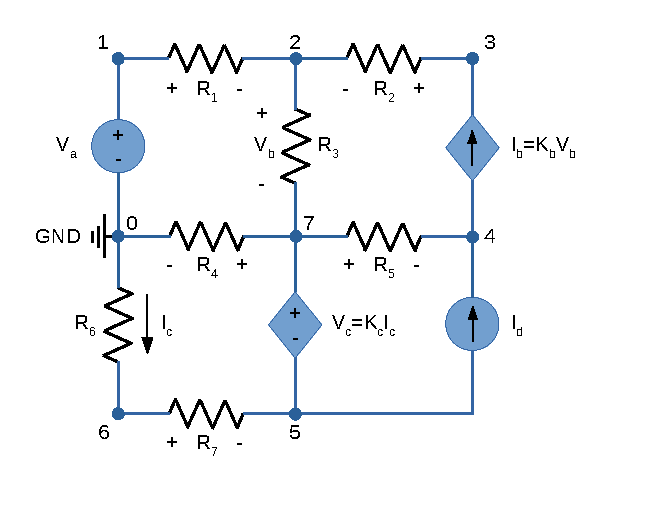
\includegraphics[width=1\linewidth]{circuit.pdf}
\caption{Circuit}
\label{fig:circuit}
\end{figure}

\newpage


\section{Theoretical Analysis}
\label{sec:analysis}

\par In this section, we will analyse our theoretical model of the AC/DC converter in terms of the DC output voltage (V_O) and the deviation from this DC value, the AC component (v_o). Our goal is to maximize the merit function given by:

\begin{equation}
M=\frac{1}{cost*(ripple(v_O)+average(v_O-12)+10^{-6}}
  \label{eq:merit}
\end{equation}
With cost given by:
\begin{equation}
M=\frac{Sum of the resistors}{1000}+\frac{Capacity}{10^{-6}}+Num_diodes*0.1
  \label{eq:cost}
\end{equation}
 
\par To maximize it we should obtain small deviations from V_O (small riplle) and obtain a V_O closer to $12V$, wich is the output voltage required. At the same time, we must reduce the cost of the circuit, by reducing the number of components and their values. We concluded that the following values were the ones that maximize this function: $C=920\miuF , R_e=920k\Omega , R_v=3.3k\Omega$.
 
\subsection{Transformer and full wave bridge rectifier}
\label{subsec:full_wave_rectifier}

\par For the first part of the circuit we used a transformer that converts the input voltage $v_S=230cos(\omega*t) V$, with $\omega=2\pi*50$, to a voltage with the same frequency and a amplitude of $230.1V$. Thus, the number of spirals for the transformer was $N=\frac{N_1}{N_2}=1.000434783$.

\par After that, we introduced a full wave rectifier circuit that converts the negative values to positive ones, so the peaks of the sinusoidal voltage appear with the double of the original frequency. Thus, the voltage that enters the envelope detector is $v_3=\abs*{230.1cos(\omega*t)}$. To do that, we use a circuit with 4 diodes (between nodes 0, 1, 2 and 3) which ensures that the output voltage is always positive, because they only conduct current in the forward active region.
\par In that way, one can reduce the ripple in the envelope detector circuit, as we will se in the next chapter.

\subsection{Envelope Detector}
\label{subsec:env}

\par The main purpose of the envelope detector is to obtain a voltage that follows the peaks of the input voltage, achieving much smaller AC components. We can distinguish 2 phases of operation, considering the ideal diode model:

\begin{itemize}
  \item When the diode is on, the envelope voltage $v_4$ is equal to $v_3$. This happens for $T_{ON}<t<T_{OFF}$, every period. 
  \item When the diode is off, it blocks the current, and the voltage in the capacitor starts discharging throuth the resistor $R_e$. The equation to compute the voltage when the diode is off is:
  \begin{equation}
v_4=230.1cos(2*\omega*T_{OFF})*e^{-\frac{t-T_{OFF}}{R_e*C}
  \label{eq:exp}
\end{equation}
\end{itemize}

 \par For computing $T_{OFF}$ we used the equation
 
  \begin{equation}
T_{OFF}=\frac{1}{2\omega}*atan(\frac{1}{2\omega*R_e*C}
  \label{eq:toff}
\end{equation}
Then we can solve the implicit equation for $T_{ON}$
\begin{equation}
v_3(T_{ON})=230.1cos(2*\omega*T_{OFF})*e^{-\frac{T_{ON}-T_{OFF}}{R_e*C}
  \label{eq:ton}
\end{equation}

\par Notice that the envelope output voltage is defined by branches. We computed the DC value of $v_4$ as $V_4=mean(v_4)$, and the ripple is the maximum deviation $ripple_envelope=max(v_4)-min(v_4)$. This ripple is reduced by doubling the frequency in the full wave bridge rectifier, because the difference between $T_{ON}$ and $T_{OFF}$ is shorter. In this table we present the values for the DC component and the ripple:

\begin{tabular}{|l|r|}
    \hline    
    {\bf Name} & {\bf Value (V)} \\ \hline
    $Ripple_{envelope}$ & $0.002240$ \\ \hline 
$Average_{envelope}$ & $22.498882$ \\ \hline 

  \end{tabular}
  \caption{Output DC voltage and ripple for the envelope detector.}
  \label{tab:env}
\end{table} 

The next plot shows the rectified voltage, $v_3$, and the envelope output voltage covering the peaks, $v_4$. 

\begin{figure}[H] \centering
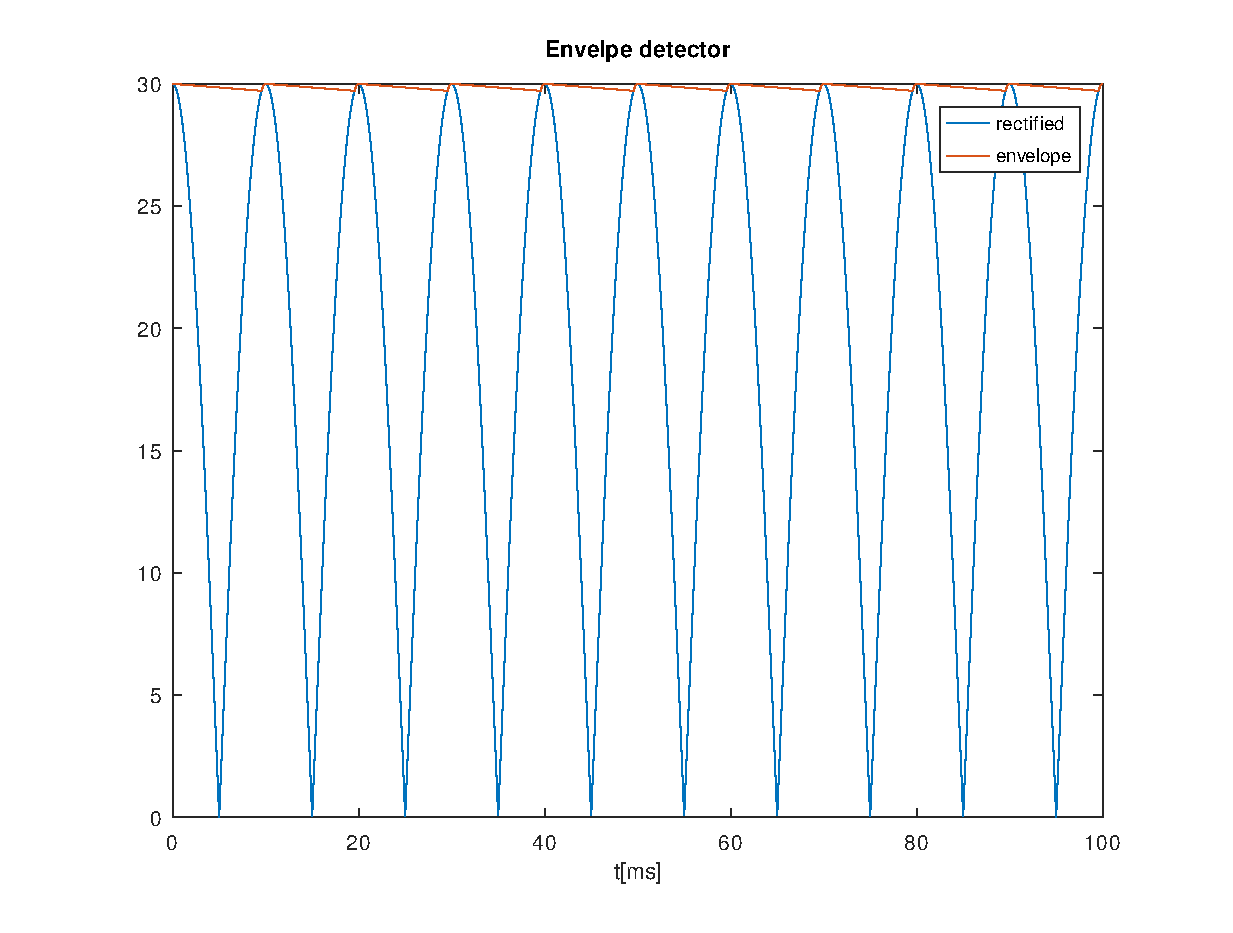
\includegraphics[clip, trim=1.3cm 1.3cm 0cm 7cm, width=0.6\linewidth]{venvlope.eps}
\caption{Rectified and envelope voltages in function of time.}
\label{fig:env}
\end{figure}

\subsection{Voltage regulator}
\label{subsec:reg}

\par The next stage is the voltage regulator, composed by 17 diodes and a resistor $R_v$. The diodes impose a DC output voltage, $V_O$, close to 12V, that was our goal to maximize the merit equation \ref{eq:cost}. By using a large resistor, we apply a voltage division in incremental terms. Therefore, one can reduce the AC component of the output voltage, $v_4$, and his ripple. We did an operating point and incremental analysis on this part of the circuit, assuming that the AC component of $v_4$ is already small.

\par To compute the operating point, we circulate the mesh composed by the diodes and the resistor $R_v$ and obtained the following equation (using only the DC component of the voltages):

\begin{equation}
 -V_4+IS*Id*R2+V_O=0
  \label{eq:reg_mesh}
\end{equation}
 
 \par Where $Id$ is the DC component of the current that passe throuth the diodes, giver by:
 
 \begin{equation}
 I_d=I_S*e^{\frac{V_O}{17*\eta*V_T}
  \label{eq:Id}
\end{equation}
 
 \par $I_S$, $\eta$ and $V_T$ are constants for the diode model used. Solving this implicit equation with Newton-Raphson methods one can obtain the DC output $V_O$, which we want to be close to 12V.  
 
 \par For the incremental analysis, we computed the incremental resistor of the 17 diodes:
 
 \begin{equation}
 r_d=\frac{\eta*V_T}{I_S*e^{\fracc{V_{ON}}{\eta*V_T}}
  \label{eq:rd}
\end{equation}

\par Where $V_{ON}$ is the threshold voltage to achieve the active region of an ideal diode model, wich we can estimate as $V_{ON}=\frac{V_O}{17}$. Using this method, instead of chosing a fixed $V_{ON}$, one can reproduce with less error the DC output given by the simulation.





\section{Simulation Analysis}
\label{sec:simulation}

\subsection{Audio Amplifier Simulation}
\label{subsec:amp_simulation}
\par In this section we simulate an audio amplifier through the NGspice tool. Our goal is to simulate the audio amplifier using two different kinds of transistors (NPN and PNP). It is our objetive to measure the output voltage gain in the passband and the lower and upper 3dB cut off frequencies, as well as the input and output impedances.

\par  \textbf{Important note:} Beyond modelling and analysing the circuit provided, one of the goals of this laboratory assignment is to maximize the merit, which is computed according to the following formula:
\begin{equation}
M = \frac{\text{voltageGain}*\text{bandwidth}}{\text{cost}*\text{lowerCutoffFreq}}
\end{equation}

Therefore, it was our intention to obtain the best value for this parameter,using each of the variables in order to maximize it, wich means that we have not tried to improve each of those separately, but as a all.
In order to do it we used the values indicated the following values of the components: $R_{B1}=79k\Omega$, $R_{B2}=9.2k\Omega$, $R_{C1}=2.4k\Omega$, $R_{E1}=150\Omega$, $R_{E2}=320\Omega$, $C_{i}=5uF$, $C_{b}=270uF$ and $C_{o}=120uF$.   
  

\begin{table}[H]
  \centering
  \begin{tabular}{ | m{11cm} | m{3cm}| } 
    \hline    
    {\bf Merit} & {\bf Value} \\ \hline
    Merit & 1.75991E-10\\ \hline
Cost & 673324 MU\\ \hline

  \end{tabular}
  \caption{Merit Calculation}
  \label{tab:merit}
\end{table}

\subsection{Output Voltage Gain}
\label{output_gain}
\par In order to measure the output voltage gain, we used Ngspice's \textit{measure} function to determine the maximum value of the output voltage. By definition the gain is the magnitude coefficient between the output voltage and the input voltage. In this particular case, the input voltage has a magnitude of 1V, wich means that we can reduce the calculation of the gain phase and magnitude to the output voltage.

 In the following table, we present the maximum magnitude of the gain (v(out)), in decibels:
 
\begin{table}[H]
  \centering
  \begin{tabular}{|l|r|}
    \hline    
    {\bf Output Voltage Gain} & {\bf Value} \\ \hline
    Output Voltage Gain dB & 266.369\\ \hline
Central Freq & 949.276\\ \hline
Low CO Freq & 453.95\\ \hline
Up CO Freq & 1985.08\\ \hline
Gain Deviation & 166.369\\ \hline
Gain Deviation dB & 8.50966\\ \hline
Central Freq Deviation &50.724\\ \hline
Bandwidth & 1531.13\\ \hline

  \end{tabular}
  \caption{Maximum Gain Magnitude, in dB}
  \label{tab:gain}
\end{table}



\subsection{Frequency response}
\label{frequency_response}
In this subsection, the same function as in the subsection \ref{output_gain} (\textit{measure}) was used to compute the value of the lower and upper 3db cut off frequencies, which allowed the calculation of the bandwidth, which is the difference of the two variables previosuly mentioned. The results obtained are shown in the table bellow:

\begin{table}[H]
  \centering
  \begin{tabular}{|l|r|}
    \hline    
    {\bf Variable} & {\bf Value [Hz]} \\ \hline
    low & 8.880418e+03\\ \hline
up & 1.603742e+06\\ \hline
bandwidth & 1.594862e+06\\ \hline

  \end{tabular}
  \caption{Lower and Upper Cut off Frequencies and Bandwidth, in Hz}
  \label{tab:frequency_response}
\end{table}



In order to compare and understand the evolution of the circuit from the gain stage to the output stage we firtly show the magnitude and the the phase plots in the collector node (the output of the gain stage) and then the same quantities regarding the output stage:

\begin{figure}[H] \centering
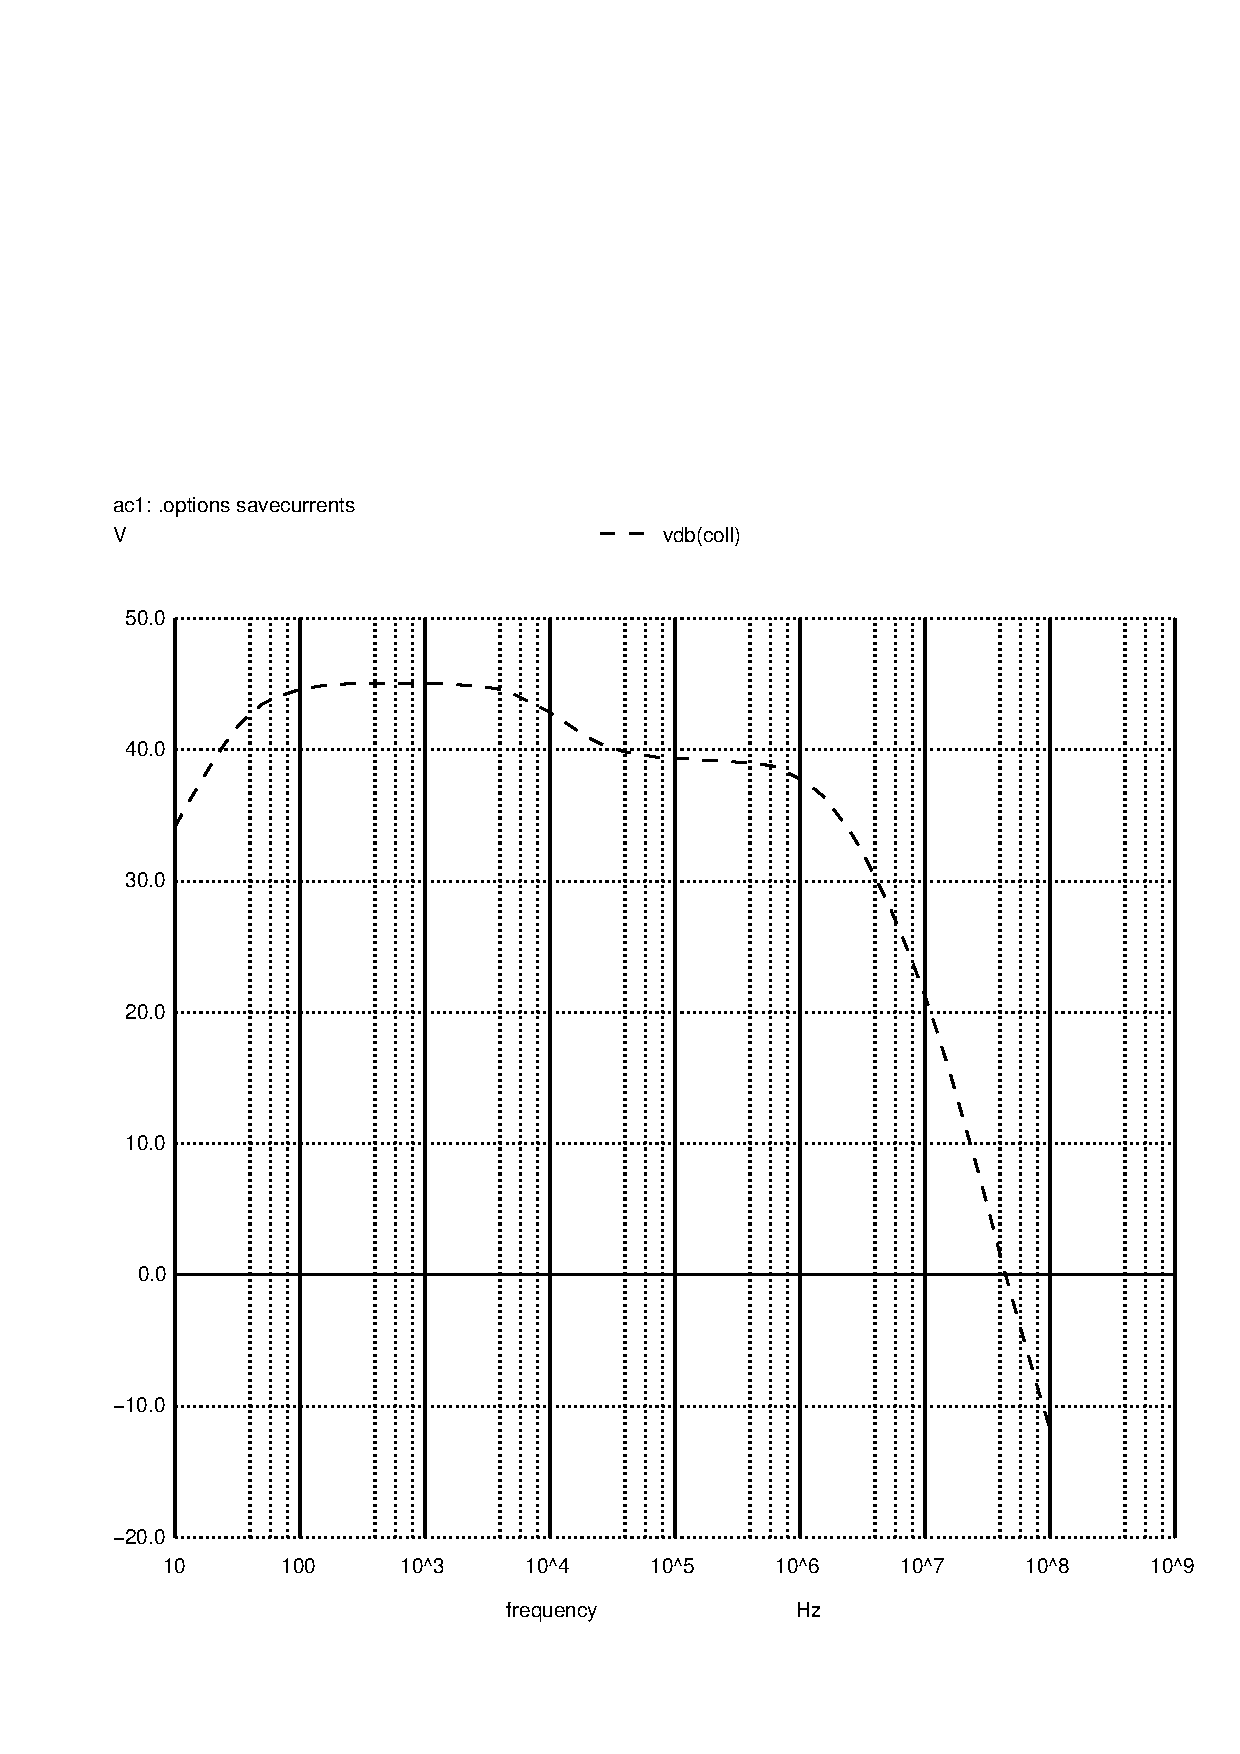
\includegraphics[clip, trim=1.3cm 1.3cm 0cm 7cm, width=0.6\linewidth]{vcolldb.pdf}
\caption{v(coll) magnitude, in dB}
\label{fig:voutdb}
\end{figure}

\begin{figure}[H] \centering
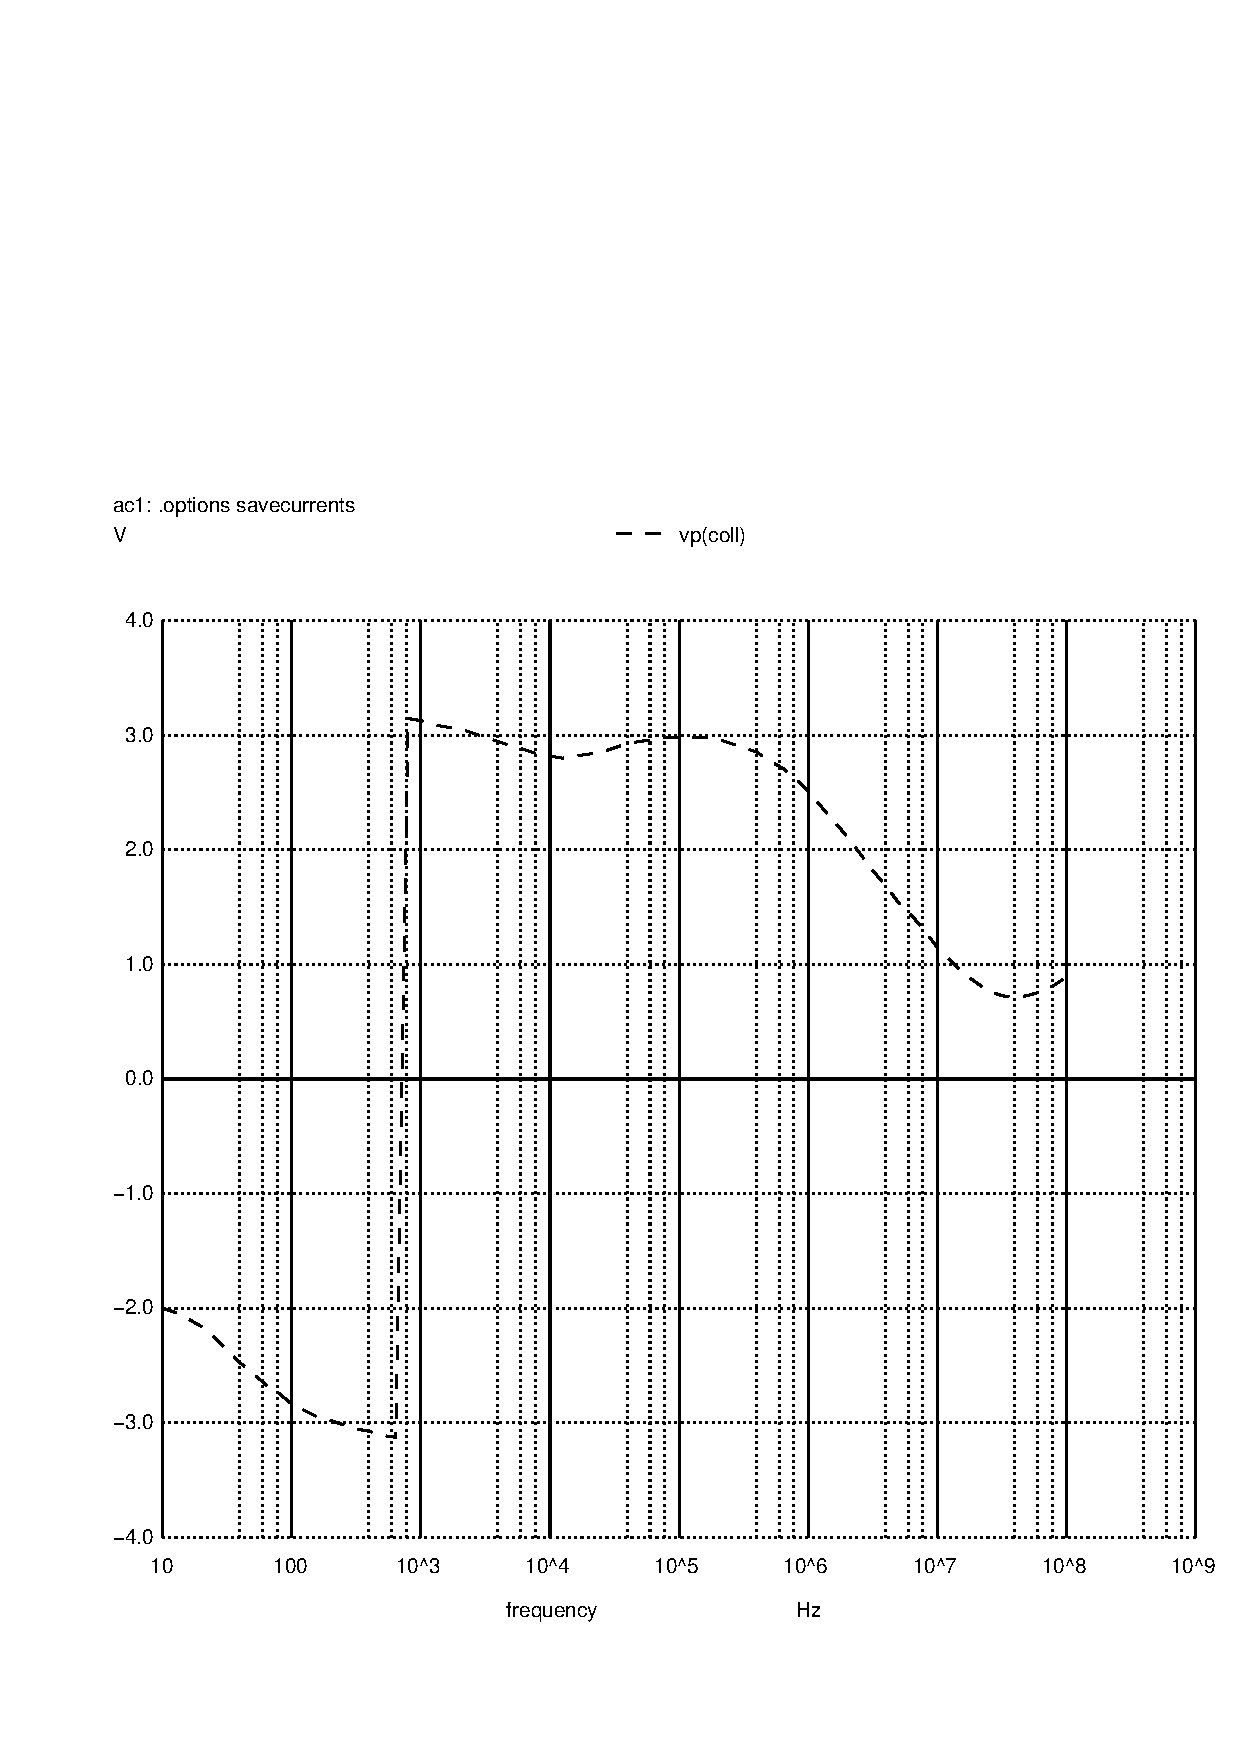
\includegraphics[clip, trim=1.3cm 1.3cm 0cm 7cm, width=0.6\linewidth]{vcollp.pdf}
\caption{v(coll) phase, in rad}
\label{fig:voutp}
\end{figure}


 Next, we present the graphical representation of both the magnitude and the phase frequency response at the output stage:
 

\begin{figure}[H] \centering
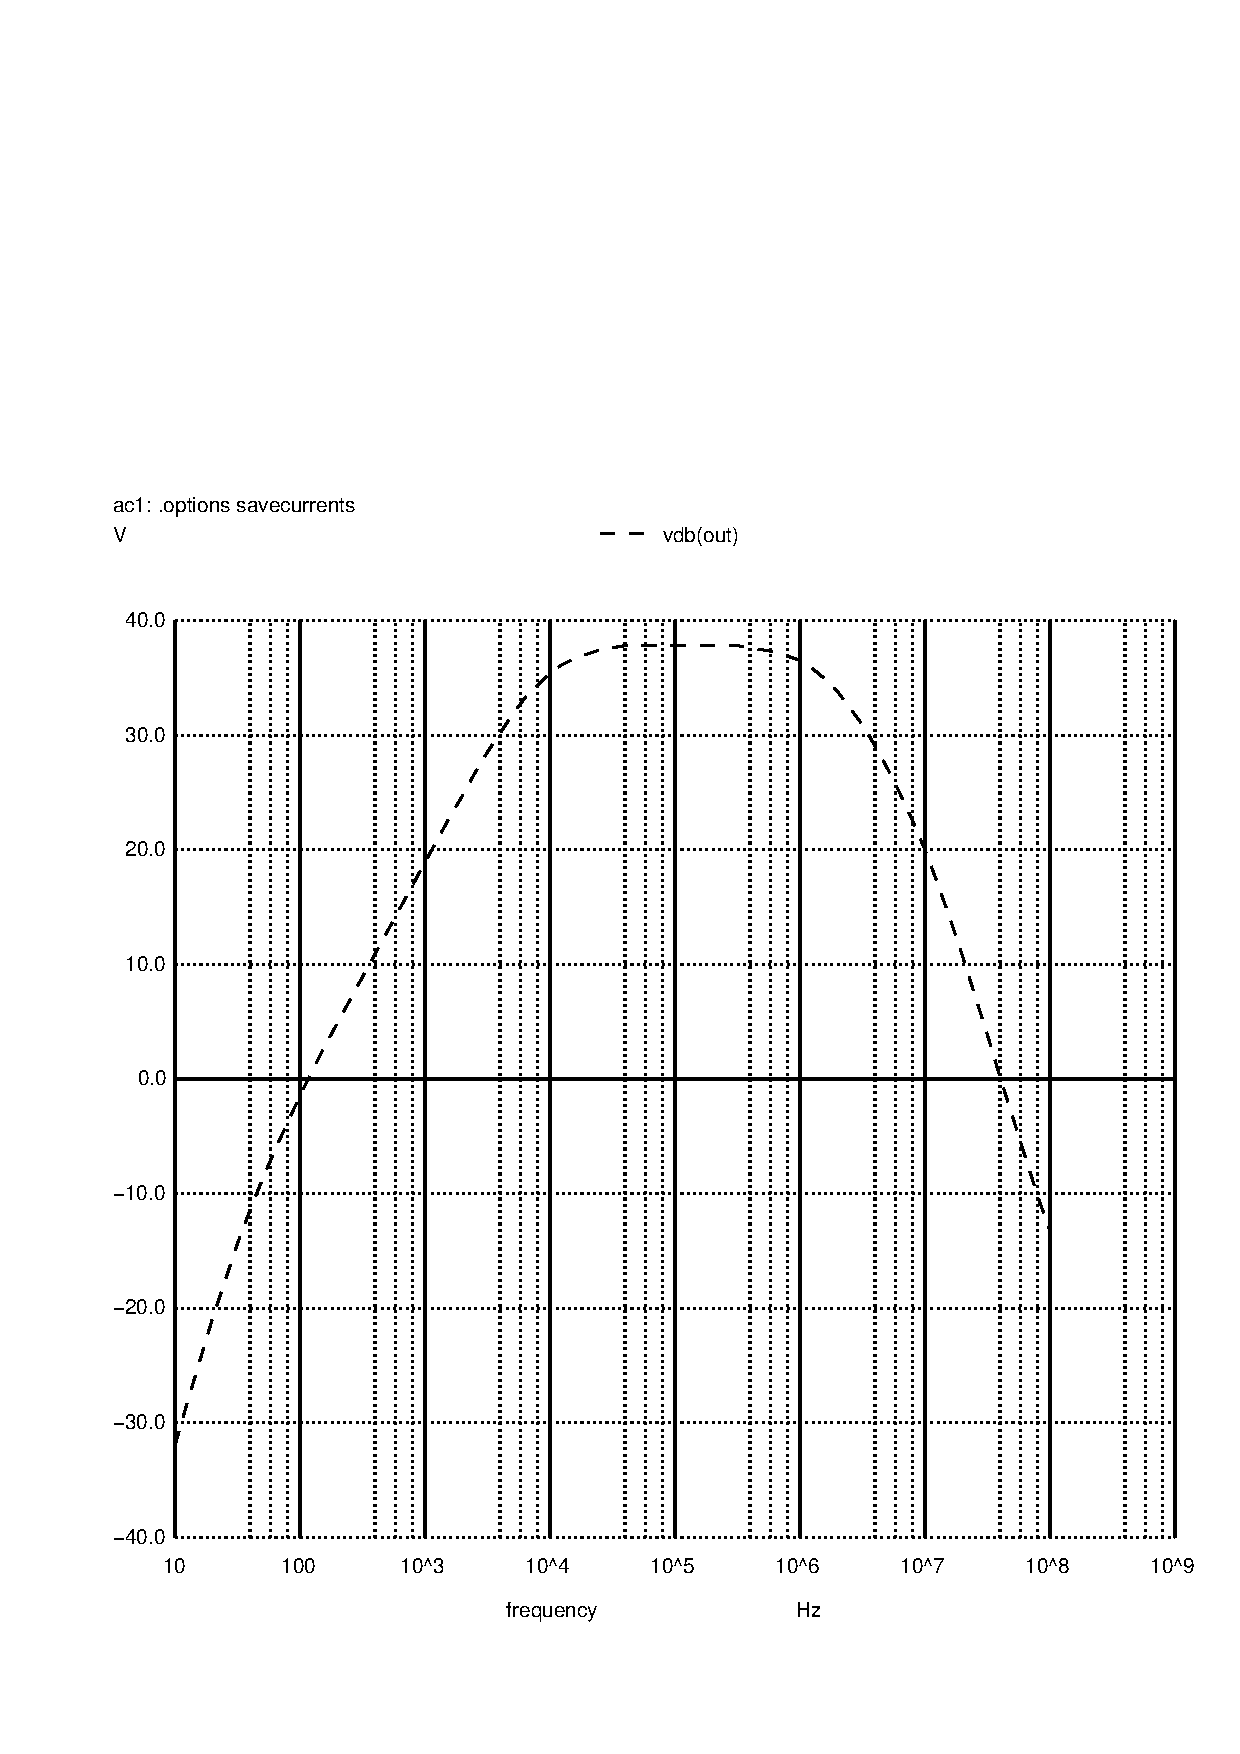
\includegraphics[clip, trim=1.3cm 1.3cm 0cm 7cm, width=0.6\linewidth]{voutdb.pdf}
\caption{Gain / v(out) magnitude, in dB}
\label{fig:voutdb}
\end{figure}

\begin{figure}[H] \centering
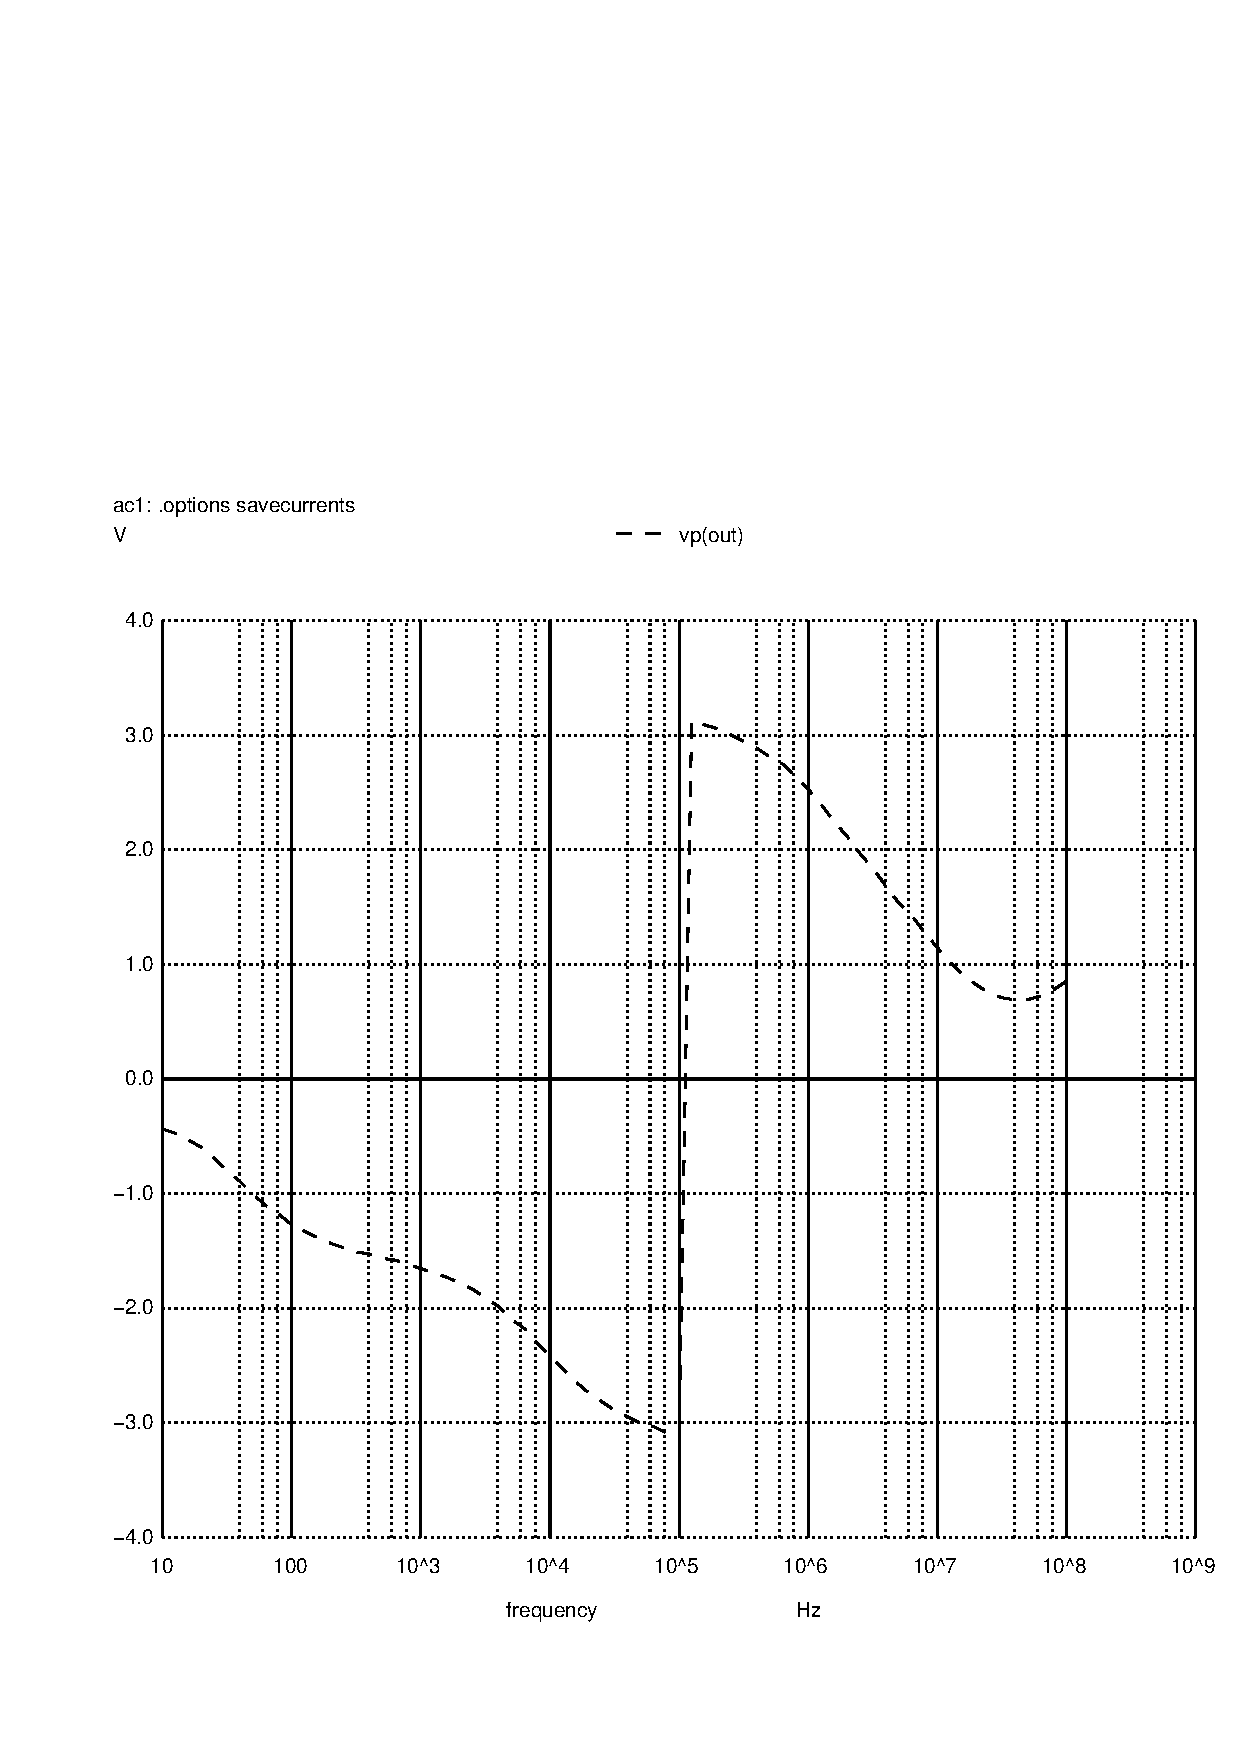
\includegraphics[clip, trim=1.3cm 1.3cm 0cm 7cm, width=0.6\linewidth]{voutp.pdf}
\caption{Gain / v(out) phase, in rad}
\label{fig:voutp}
\end{figure}


\subsection{Impedances}
\label{impedances}
Finally, in this subsection the input impedance and the output impedance are presented. We can verify from them values that we achieved the goal of having a high input impedance and a low output impedance, wich allow to obtain a better amplifier:


\begin{table}[H]
  \centering
  \begin{tabular}{|l|r|}
    \hline    
    {\bf Input Impedance} & {\bf Value [S]} \\ \hline
    zi & 5.638527e-01,-8.44302e-02\\ \hline

  \end{tabular}
  \caption{Input Impedance, in Siemens}
  \label{tab:input_z}
\end{table}


\begin{table}[H]
  \centering
  \begin{tabular}{|l|r|}
    \hline    
    {\bf Output Impedance} & {\bf Value [S]} \\ \hline
    zo & -1.00554e+01,1.184265e+00\\ \hline

  \end{tabular}
  \caption{Output Impedance, in Siemens}
  \label{tab:output_z}
\end{table}





\section{Conclusion}
\label{sec:conclusion}

After the theoretical analysis, the simulation and the results' comparison, it can be
concluded that the design and analysis of the amplifier circuit, presented in Figure-\ref{fig:circuit}, has been accomplished.\par

There were performed both a theoretical and a simulation analysis, where the importance of this kind of circuits became noticeable. This laboratory assignment allowed us to contact with a more realistic problem in a way that its goal forced us to integrate all of our knowledge acquired untill this moment, and allowed us to understand what is in stake when we need to use models to aproximate a circuit. Beyond this, the circuit analysed is very usefull on our daily life.
We managed to obtain a good value of gain, wich means that the amplification was successfull
Concluding, we were able to achieve the proposed objective and became more aware of the real context of the applications of this course lectures.

%\cleardoublepage

% ----------------------------------------------------------------------
%  Bibliography
% ----------------------------------------------------------------------
%\addcontentsline{toc}{section}{\bibname}
%\bibliographystyle{abbrvunsrtnat} % <<<<< SELECT IF USING REFERENCES BY NUMBER (CITATION ORDER)
%\bibliography{../../../BIBfile.bib}

% ----------------------------------------------------------------------
\end{document}
% ----------------------------------------------------------------------
